{\color{indiagreen}\subsection{Vsiljeno nihanje}}
Ko na nihalo delujemo s periodično silo.\\
\begin{align*}
	\nu &\dots \text{frekvenca sile}\\
	\nu_0 &\dots \text{lastna frekvenca nihala}\\
\end{align*}
\textbf{Resonančna} krivulja je aplituda v povezavi z vzbujevalno frekvenco.\\
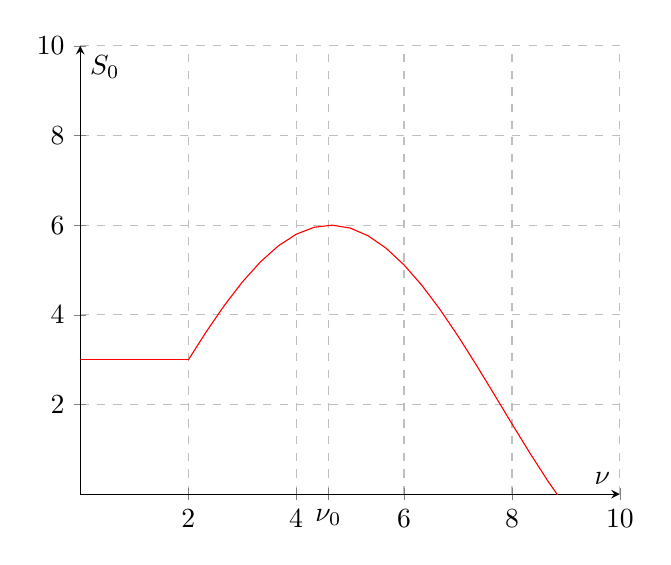
\begin{tikzpicture}
	\begin{axis}[
	    xlabel={$\nu$},
	    ylabel={$S_0$},
	    xmin=0, xmax=10,
	    ymin=0, ymax=10,
	    xtick={0,2,4,4.6,6,8,10},
	    ytick={0,2,4,6,8,10},
	    xticklabels={0,2,4,$\nu_0$,6,8,10},
	    ymajorgrids=true,
	    xmajorgrids=true,
	    grid style=dashed,
	    axis lines=middle,
	]
	\addplot[domain=0:2,red] {3};
	\addplot[domain=2:10,red] {2 + 4 * sin(deg(x/2 - 0.75))};
	\end{axis}
\end{tikzpicture}\\
\begin{align*}
	S_0 &\dots \text{Na grafu predstavlja amplitudo.}\\
	\nu &\dots \text{Na grafu predstavlja vzbujeno $\nu$.}\\
	\nu_0 &\dots \text{Vrh je ko sta obe enaki.}\\
	\nu &<<\nu_0 \dots \text{Amplituda se ne spremeni.}\\ 
	\nu &=\nu_0 \dots \text{Amplituda se močno poveča, \textbf{resonanca}.}\\
	\nu &>>\nu_0 \dots \text{Amplituda se močno spremeni.}\\
\end{align*}
